\def\p{\text{p}}
\section{Higher dimensional coend calculus.}\label{sec:higher}
\epigraph{Entonces desaparecerán del planeta el inglés y el francés y el mero español. El mundo será Tlön. Yo no hago caso, yo sigo revisando en los quietos días del hotel de Adrogué una indecisa traducción quevediana (que no pienso dar a la imprenta) del {\em Urn Burial} de Browne.}{J.L. Borges, \emph{Tl\"on, Uqbar, Orbis Tertius}}
Category theory was born in 1945 when Mac Lane and Eilenberg \cite{gtone} isolated the correct definition of natural transformation between functors.

By doing this, they  introduced the paradigmatic example of a 2-category: in this precise sense then \emph{higher category theory} is a field as old as category theory itself. And yet, despite its age, it remains an area where even basic questions, burdened by an intrinsic computational difficulty, are still intricate, subtle and very challenging.

Even though for many years higher-dimensional category theory remained confined to well-defined geographical areas, the last 15 years witnessed a super-exponential growth of interest across several areas of mathematics: higher categorical structures have been recognized to lie at the heart of modern approaches to geometry \cite{toen2005homotopical}, \cite{HTT}, \cite{ben2010integral}, logic \cite{hottbook}, topology and mathematical physics \cite{Schreiber2013}; the slow but constant diffusion of a dialect which is powerful enough to encompass all these developments, and yet sufficiently simple to be studied led to the present situation and led to a fairly general ``reinterpretation'' of known theories in a new language, inspired by homotopy theory. Higher category theory and the fundamental constructions therein are hence interpreted in a homotopy-invariant way.\footnote{One of the main tenets of higher category theory is that, whatever they are, these objects live in the world of (abstract) homotopy theory. There are several ways to justify this apparently strange remark, but this margin is too narrow to contain any of them: the starting point for most of them is that the nerve functor $N_i$ (as described in \S\refbf{section:nr}) provides a fully faithful embedding $\Cat\subseteq \sSet$; the wild variety of model structures on the category of simplicial sets becomes then a tool to better understand category theory.} The process of passing from a 1-categorical (also called ``classical'' in the following) setting to an higher-categorical one can be seen as a process of ``heightening''.

Co/end calculus, as a part of the categorical toolbox, makes no exception and can be heightened (in fact, in several ways). 

The scope of the present chapter is to give a compact but lucid presentation of this ``higher co/end-fu'' (a possible translation could be \begin{CJK*}{UTF8}{bsmi}高维 端楔術\end{CJK*}). The struggle here is on two separate and opposing fields: on one side, ``ancient'' higher category theory \cite{coherence-tricat,hoffnung2011spans} with its baroque equational approach to coherence conditions is a true nightmare, both for the listener and the exposer. On the other side the ``new'' approach to higher category theory based on homotopy theory (mainly that of simplicial sets) reinterprets those very coherence conditions allowing a precious bookkeeping device, which is nevertheless often too far from the taste of some practitioners of categorical algebra.

This simple observation does not distance the author from the current fashion and the current belief: the ``homotopical'' approach to higher categories proved to be a valid tool to actually \emph{do} beautiful mathematics, and speaks a subtle and intricate language, forbidden to the inhabitants of the 1-dimensional world. Nevertheless, we feel this is the right place to clarify our philosophical position.

At the moment of writing this note we (as a community) witness several attempts to acquire a deeper understanding of the landscape of current mathematics at the level of its fundamental architecture; category theory, with its indisputable unification power, can be encoded in homotopy theory, and this is part of a turnaround which takes the notion of \emph{homotopy} as a primitive idea interacting with the similarly primitive notion of \emph{structure} and \emph{operation} on a space (seen from this perspective, sets are discrete groupoids and hence particular cases of topological spaces): there is a growing feeling that any attempt to rewrite a piece of ``old'' mathematics turning it into an ``homotopically meaningful'' statement is, in a suitable sense, a piece of higher category theory.

This is a peculiar, transitional moment in pure mathematics; several generations used to think in terms of set theory resist the revolution, thinking that the homotopy groups of spheres form a too complicated object to ``lie at the foundation'' of current mathematics. This point of view in some sense indisputable, and yet the author feels that it underlies a subtle epistemological problem (what is ``simple mathematics''? What has, and what has not, the right to be considered a primitive entity? What is, in the end, the ``right'' primitive entity to choose for a foundation of mathematics?) which has no hope to be solved ever (so a fortiori, not in the space of this paragraph).

At the very least, this suggests that the extremely positive attitude towards the outreach of category theory among the barbarians\footnote{The word here only means ``the people living outside the \emph{polis} of category theory'', without any pejorative meaning.} must be taken with a grain of salt. Categorical jargon gets more and more acknowledged as more and more applications for it are found, and yet it still suffers from a certain ostracism by some parts of the mathematical community. This is not, or at least not completely, their fault, and results in a generalized discomfort. 

Together with the development of the language, nobody cared about a complementary development of self-contained presentations, as elementary as possible, forgetting how this is essential for a rapid and `` healthy '' diffusion of good ideas. The canonical sources where higher category theory has been distilled are difficult and time-consuming readings; this leaves many people behind. The technical subtleties, the intrinsic difficulty of simplicial homotopy theory and the lack of a metatheory serving as intuition in natural language make the big picture visible only to a handful of people, often the same creators of the theory; this deters other people to collaborate. 

In this age where categorical language is expanding, it is more necessary than ever to write, to write well, and write simply, addressing to everyone. It is a deep author's conviction that by doing this the overall health of mathematical practice significantly improves, as well as the prompt and faithful diffusion of profound ideas that would otherwise be exclusively dedicated to an élite. Rather, it is the consequence of a precise historical moment and ideology. This kind of commitment, carried out in the past, allowed generations of totally unprepared students to appreciate the depth of rich and complex definitions (now for real, undoubtedly, a root of the mathematical language essential to every practitioner).

As in all ``critical'' moments --in which you carefully consider the risks and benefits of a language-shift-- we should be oriented towards ideological openness and a multilingual attitude: this simple pedagogical principle is unfortunately often forgotten by innovators of all ages.

It is difficult to foresee where the current landscape will lead us; eventually, the world will become Tl\"{o}n. All we can do until then is wait, and have fun learning something beautiful. 
\subsection{2-coends.}
% \trans{TO BE POLISHED A LOT.}
One of the most immediate generalization of co/end-fu lives in the world of 2-categories, where ``1-cells'' are allowed to be transformed by ``2-cells''. 

In view of \aprop\refbf{coends.as.colims}, to define 2-co/ends we must exploit some flavour of limit and colimit in 2-category theory: this calculus has a rather natural interpretation in terms of enriched category theory (\cite{kelly1974review} and \cite{2catlimits}, for example, offer an invaluably complete survey on this topic, but the reader should be aware that 2-category theory is \emph{not} the theory of $\Cat$-enriched categories). Here the reader is also warned that the following discussion has little or no hope to be a self-contained exposition, and instead heavily relies on classical sources as \cite{kelly1982basic,dubuc1970kan}.
\begin{notat}
As always when dealing with higher dimensional cells and their compositions, there are several ``flavours'' in which one can weaken strict commutativity: besides this strictness (where every diagram commutes with an implicit identity 2-cell filling it), there is a notion of \emph{strong} commutativity and universality, where filling 2-cells are requested to be invertible, and \emph{lax} commutativity/universality, where 2-cells are possibly non-invertible.\footnote{Obviously there are two possible choices for a direction in which a non-invertible ``laxity cell'' can go: a map endowed with a canonical 2-cell $F(g)F(f)\Rightarrow F(gf)$; the same correspondence, with 2-cells $F(gf)\Rightarrow F(g)F(f)$ is called \emph{op}lax functor. The reader will find a personal mnemonic trick to remember how this nomenclature is chosen.}
\end{notat}
The definition of \emph{lax end} of a 2-functor $S$ (given in terms of a universal \emph{lax wedge} $\omega\colon b\xto{..}S$) is the most general and less symmetric one can give (it can still be dualized to a colax coend, though!); definitions and theorems in this subsection are designed and proved in such a way to reduce to the strong and strict cases as particular examples of lax co/ends, where filling 2-cells are invertible (resp\@., identities).
\paragraph{\bf Local notation.} For the rest of the section we adopt some local conventions: first of all, we denote $\A\laxto \B$ a lax functor between two 2-categories $\A,\B$; as sketched above, this means that we have a correspondence $F_0\colon \ob(\A)\to \ob(\B)$ and a correspondence $F_1\colon \hom_1(\A)\to\hom_1(\B)$ at the level of 1-cells, such that there exist ``laxity cells'' $F(g)F(f)\Rightarrow F(gf)$ and $\id_{F_0a}\to F_1(\id_a)$, satisfying ``obvious'' coherence conditions. 

This said, 2-category theory exists in many dialects: we mainly follow a natural and auto-explicative notation based on the canonical reference \cite{2catlimits}, but we feel free to diverge from it from time to time: the operations of \emph{whiskering} of an higher cell with a lower cell is denoted with the symbol $*$, so that $F * \alpha \colon FH\Rightarrow FK$ and $\alpha*G \colon HG\Rightarrow KG$ for natural transformation $\alpha\colon H \Rightarrow K$ and suitable functors $F,G$.
\begin{definition}\label{laxwedge}
Let $S\colon \A^\opp\times \A \to \B$ be a strict 2-functor between strict 2-categories. A \emph{lax wedge} based at $S$ consists of a triple $\{b, \underline{\omega}_{\ob}, \underline{\omega}_{\hom}\}$, where $b\in \ob(\B)$ (the \emph{tip} of the wedge) and collections of 1-cells $\big\{ \omega_a\colon b\to S(a,a)\big\}$, one for each $a\in \ob(\A)$, and 2-cells $\big\{ \omega_f\colon S(a, f)\circ \omega_{a} \Rightarrow S(f, a')\circ \omega_{a'} \big\}$, in a diagram
\begin{center}
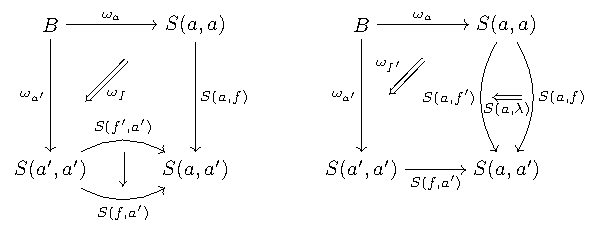
\includegraphics[scale=1]{figures/fig15}
\end{center}
These data must fit together in such a way that the following coherence axioms, expressed by the commutation and pasting of the following diagrams of 2-cells, are satisfied:
\begin{enumerate}[label=(\oldstylenums{\arabic*})]
\item The diagram of 2-cells
\begin{center}
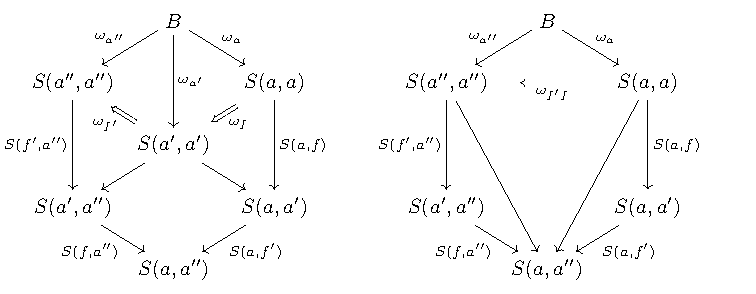
\includegraphics[scale=1]{figures/fig16}
\end{center}
is commutative for any $\lambda\colon f\Rightarrow f'$, \ie   the equation
\[
\omega_{f'}\circ (S(a, \lambda)*\omega_a) = (S(\lambda, a') * \omega_{a'})\circ \omega_f
\]
holds.
\item For each pair $a\xto{f}a'\xto{f'}a''$ of composable arrows in $\A$, the diagram of 2-cells
\begin{center}
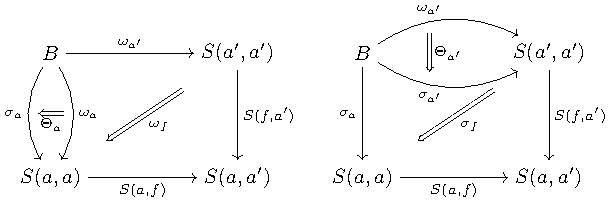
\includegraphics[scale=1]{figures/fig17}
\end{center}
is commutative, \ie   the equation
\[
(S(f, a'') * \omega_{f'})\circ (S(a, f') * \omega_f) = \omega_{f'f}
\]
holds.
\item For each $a\in\A$, $\omega_{\id_a} = \id_{\omega_a}$.
\end{enumerate}
\end{definition}
\begin{notat}
A lax wedge will be often denoted $\underline{\omega}\colon b\xto{..}S$ for short; this is evidently reminiscent of our Def\@. \refbf{extranatural} and \cite{McL}.
\end{notat}
\begin{definition}[Modification]\label{modification}
A \emph{modification} $\Theta\colon \omega\Rrightarrow\sigma$ between two lax wedges $\underline{\omega},\underline{\sigma}\colon b\xto{..}S$ for $S\colon \A^\opp\times \A \to \B$ consists of a collection of 2-cells $\{ \Theta_a\colon \omega_a\Rightarrow \sigma_a\}_{a\in \ob(\A)}$ such that the diagram of 2-cells
\begin{center}
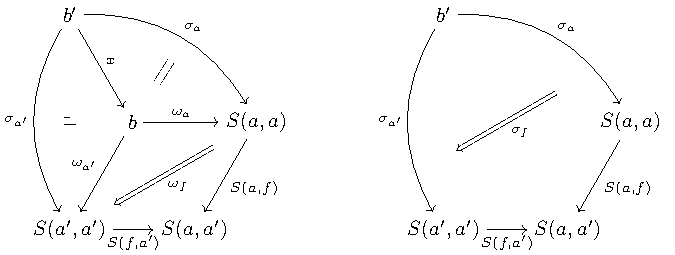
\includegraphics[scale=1]{figures/fig18}
\end{center}
is commutative, \ie 
\[
(S(a,f) * \Theta_a)\circ \omega_f = \sigma_f \circ (S(f,a') * \omega_{a'})
\]
\end{definition}
The definition of a modification is modeled on the definition of modification between (lax, if necessary) natural transformations; modifications form the 3-cells of the 3-category $2\text{-}\Cat$, whose objects are 2-categories, 1-cells are (lax, if necessary) functors, 2-cells are (lax, if necessary) natural transformations.

Modifications follow rules for ``whiskering'' which are similar to those for natural transformations and 2-cells, only in higher dimension (and in a much complicated web of relations between all the possible compositions: there are now \emph{three} possible directions in which 3-cells can be composed!).
\begin{remark}
There is another more general definition for a modification $\Theta\colon \omega\Rrightarrow\sigma$ between lax wedges having different domains, say $\{b, \underline{\omega}\}$ and $\{b', \underline\sigma\}$: it consists of a morphism $\varphi\colon b\to b'$ and a 2-cell $\lambda_a\colon \sigma_a \circ\varphi \Rightarrow \omega_a$ such that
\[
(\sigma_f * \varphi)\circ (S(a,f) * m_a) = (S(f, a') * m_{a'})\circ \omega_f
\]
(draw the corresponding diagram of 2-cells!). Nevertheless, we are not interested in this alternative definition; Def\@. \refbf{modification} entails that the set $\textsf{LFun}(b, S)$ of lax wedges $b\xto{..}S$ is a category having morphisms precisely the modifications $\Theta\colon \underline\omega\Rrightarrow \underline\sigma$, and the correspondence $\beta_S\colon b\mapsto \textsf{LFun}(b,S)$ is functorial. The definition of \emph{lax end} for $S$ relies on the representability of this 2-functor.
\end{remark}
\begin{definition}[Lax end of $S$]
Let $S\colon \A^\opp\times \A \to \B$ be a 2-functor; a lax wedge $\underline\omega\colon b\xto{..} S$ is called the \emph{lax end} of $S$, and denoted $\twoint_a S(a,a) \xto{..} S$ if for any other lax wedge $\underline\sigma\colon b'\to S$ there exists a single 1-cell $x\colon b'\to b$ between the tips of the wedges such that
\[
\omega_a \circ x = \sigma_a, \notag\qquad\qquad
\omega_f * x = \sigma_f
\]
\ie the diagram of 2-cells
\begin{center}
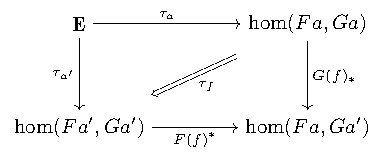
\includegraphics[scale=1]{figures/fig19}
\end{center}
commutes, and if every modification $\Theta\colon \underline\sigma\Rrightarrow \underline\sigma'$ induces a unique 2-cell $\lambda\colon x\Rightarrow x'$ ($x'$ is the arrow induced by $\underline\sigma'$) in such a way that
$\lambda * \omega_a = \Theta_a$. This realizes the isomorphism of categories between lax wedges $b \xto{..} S$ and $\B(b, \twoint_a S(a,a))$.

We denote, with an evident and harmless abuse of notation, \[
B_S = \twoint_a S(a,a).
\]
\end{definition}
\begin{remark}
The notation chosen for $\twoint_a S$ has a meaning: ideally, the $n$-co/end operation is depicted by an integral symbol (accordingly super- or subscripted) overlapped by an $2^n$-agon; in this way, a 2-end has the right to be denoted as a ``square-integral'' $\twoint$, and a $\infty$-end (see \adef\refbf{infend}) should be denoted as a $\infint$ symbol, the circle being a polygon with an infinite number of sides.
\end{remark}
\subsubsection{\bf Lax co/end calculus.}
Several \emph{kata} of coend-fu proved in our \S\textbf{1} and \S\textbf{2} remain true after a proper ``laxification'', justifying the intuition of lax co/ends as the right 2-categorical generalization of strict co/ends. We collect the most notable examples of this phenomenon in the rest of the section; the content of \refbf{laxyonedaninja} surely deserves a special mention, as well as other remarks chosen to convey a sense of continuity and analogy. In \refbf{laxyonedaninja} we prove that the lax counterpart of the ninja Yoneda lemma \refbf{ninjayo} provides a reflection (using coends) and a reflection (using ends) of the category of strong presheaves into the category of lax presheaves.
\begin{example}\label{commaobj}
The \emph{comma objects} $(f/g)$ \cite{Gray} of a 2-category $\B$ can be identified with the lax end of functors $\mathbf{2}^\opp\times\mathbf{2}\to \B$ choosing the two 1-cells $f,g$; this is a perfect analogy of Exercise \textbf{1}.\refbf{ispull}, in view of the characterization of the comma object $(f/g)$ as a lax pullback in $\Cat$.
\end{example}
\begin{example}\label{laxnat}
If $F,G\colon \A\to \B$ are 2-functors, then the lax end of the functor
\[
\B(F,G)\colon \A^\opp\times \A\to \Cat
\]
is given by the formula
\[
\twoint_a \B(Fa,Ga)\cong \textsf{LFun}(\A, \B)(F,G)
\]
where $\textsf{LFun}(\A, \B)(F,G)$ is the set of lax natural transformations between lax functors $F,G\colon \A\to \B$ defined in \cite{Gray}.
\end{example}
\begin{proof}
A lax wedge for the 2-functor $(a,a')\mapsto \hom(Fa, Ga')$ amounts to a square
\begin{center}
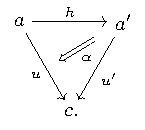
\includegraphics[scale=1]{figures/fig20}
\end{center}
filled by a 2-cell $\tau_f\colon G(f)_* \circ \tau_a \Rightarrow F(f)^* \circ \tau_{a'}$. Each of the functors $\tau_a\colon \cate E\to \hom(Fa, Ga)$ sends $e\in \cate E$ into an object $\tau_a(e)$ such that
\[
G(f)\circ \tau_a(e) \overset{\tau_f}\Longrightarrow \tau_{a'}(e)\circ F(f)
\]
which is precisely what is needed to show that the correspondence $e\mapsto \{\tau_a(e)\}_{a\in \A}$ factors through $\textsf{LFun}(\A,\B)(F,G)\subseteq \prod_{a\in\A}\hom(Fa, Ga)$.
\end{proof}
Lax natural transformations $\eta\colon F\laxto G$, described as the lax end above, can also be characterized as \emph{lax limits} in the enriched sense: this motivates the search for a description of lax co/ends which is analogue to our \refbf{coends.as.colims}, where instead of strict co/equalizers we use \cite{2catlimits}'s notion of \emph{co/inserter}.

For the ease of the discussion, we recall now how these lax limits are defined (see \cite[\S\textbf{4}]{2catlimits}):
\begin{definition}
Let $f,g\colon x\to y$ be two parallel 1-cells in the 2-category $\C$; the \emph{inserter} $\textsf{Ist}(f,g)$ is defined as a pair $(p,\lambda)$ where $p\colon \textsf{Ist}(f,g)\to x$ is a 1-cell in $\C$ and $\lambda\colon fp \Rightarrow gp$ is a 2-cell, universal with respect to the property of connecting $fp, gp$: this means that whenever we are given a diagram
\begin{center}
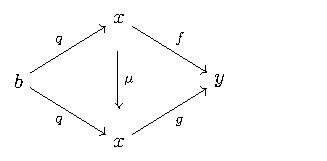
\includegraphics[scale=1]{figures/fig6}
\end{center}
this can be split as the whiskering
\begin{center}
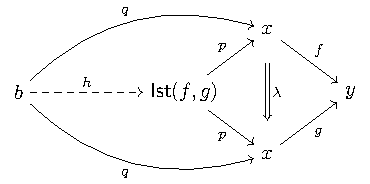
\includegraphics[scale=1]{figures/fig7}
\end{center}
for a unique 1-cell $h\colon b\to \textsf{Ist}(f,g)$ in $\C$: this means, again, that $ph=q$ and $\lambda * h = \mu$.
\end{definition}
This remark motivates the search for a description of lax co/ends as lax co/limits, on the same lines of our Remark \refbf{is.a.colim}; this is the content of Prop\@. \refbf{lax.is.wcolim} in this section.

Moreover, as an analogue of the claim for 1-dimensional co/ends, we will prove that the lax co/end of a functor which is mute in a variable coincides with the lax co/limit of the same functor restricted to the unmuted component:
\begin{remark}[Commutation of lax limits]\label{laxlimcommute}
Strict limits are obviously particular cases of lax limits; since the classical argument, slightly modified to encompass the presence of non trivial laxity  cells, applies to show that lax limits commutes with lax limits (in an obvious sense which we invite the keen reader to make precise), we obtain that lax co/limits (and lax co/ends) commute with strict co/limits (and lax co/ends).
\end{remark}
This simple remark will be used all along the present section, and in a similar way we can deduce the ``lax Fubini rule'' for iterated lax co/ends: here is an ordered exposition for these results.
\begin{proposition}[Co/ends of mute functors]
Suppose that the 2-functor $S\colon \A^\opp\times\A \to \B$ is mute in the contravariant variable, \ie  that there is a factorization $S = S'\circ p\colon \A^\opp\times\A \xto{p} \A \xto{S'} \B$
\[
\twoint_a S(a,a)\cong q\underleftarrow{\dashlim} S'
\]
hence every lax co/limit can be computed as a lax co/end.
\end{proposition} 
\begin{example}
As a particular example of this, if $\A$ is locally discrete (\ie identified with a locally small 1-category) and if the functor $S'\colon \A\to \B$ is constant, \ie $S'(a) \equiv b$ for each $a\in \A$, then $\twoint_a S$ is called \emph{cotensor} of $b$ by $\A$ and is denoted $b\pitchfork \A$.
\end{example}
\begin{theorem}[Parametric lax Ends]
Whenever a functor $F\colon \A^\opp\times \A\times \B\to \C$ is defined, and the lax end $\twoint_a F(b, a,a)$ exists for every $B\in \B$, then $b\mapsto \twoint_a F(b, a,a)$ extends to a 2-functor $\B\to \C$ which has the universal property of the lax end of its mate $\hat F\colon \A^\opp\times \A \to \C^{\B}$ under the obvious adjunction.
\end{theorem}
\begin{theorem}[Fubini rule for lax co/ends]\label{laxfubini}
If one among the following lax ends exists, then so does the others, and the three are canonically isomorphic:
\[
\twoint_{b,c}T(b,c,b,c)\qquad \twoint_b\left(\twoint_c T(b,c,b,c)\right) \qquad \twoint_c\left(\twoint_b T(b,c,b,c)\right)
\]
\end{theorem}
\begin{corollary}[Fubini rule for lax co/limits]
Lax limits commute: if $T\colon \B\times \C\to \D$ is a 2-functor, we have
\[
	q\underset{b\in \B}{\underleftarrow{\dashlim}}\;
	q\underset{c\in \C}{\underleftarrow{\dashlim}}\; T(b,c)
	\cong 
	q\underset{c\in \C}{\underleftarrow{\dashlim}} \; 
	q\underset{b\in \B}{\underleftarrow{\dashlim}} \;  T(b,c).
\]
\end{corollary}
\subsubsection{\bf The lax ninja Yoneda lemma.}\label{laxyonedaninja} The lax analogue of Prop\@. \refbf{ninjayo} acquires an extremely particular flavour in this context, since it is the gist of an argument which shows the co/reflectivity of the category of \emph{strict} presheaves $\C^\opp\to \Cat$ in the category of lax presheaves $\C^\opp\laxto \Cat$: there is a diagram of adjoint 2-functors
\begin{center}
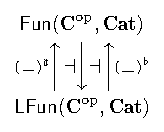
\includegraphics[scale=1]{figures/fig8}
\end{center}
This means that for each strict 2-functor $H\in \textsf{Fun}(\C^\opp, \Cat)$ there are two natural isomorphisms
\begin{gather}
\textsf{Fun}(\C^\opp, \Cat)(H, F^\bemo) \cong \textsf{LFun}(\C^\opp, \Cat)(H,F),\notag \\
\textsf{Fun}(\C^\opp, \Cat)(F^\diesis, H)\cong \textsf{LFun}(\C^\opp, \Cat)(F,H)
\end{gather}
where the functors $F^\bemo$ and $F^\diesis$ are defined by the lax coends
\[
F^\diesis \cong \twoint^a \C(\firstblank,a)\times Fa \qquad\qquad
F^\bemo \cong \twoint_a Fa^{\C(a,\firstblank)}.
\]
\begin{proof}
The proof exploits Example \refbf{laxnat} as well as the commutation of co/ends and lax co/ends, the preservation of lax co/ends by the hom functor, and the strict ninja Yoneda lemma:
 \begin{align*}
 \textsf{Fun}(\C^\opp,\Cat)(H, F^\bemo) & = \int_c \Cat(Hc, F^\bemo c) \\
& = \int_c \Cat \left(Hc, \twoint_a \Cat(\C(a,c), Fa) \right)\\
 & \cong \int_c \twoint_a \Cat(Hc, \Cat(\C(a,c), Fa)) \\
 & \cong \twoint_a \int_c \Cat(Hc\times \C(a,c), Fa) \\
 & \cong \twoint_a \Cat\left( \int^c Hc \times \C(a,c), Fa \right)\\
 & \cong \twoint_a \Cat(Ha, Fa) \overset{(\refbf{laxnat})}= \textsf{LFun}(\C^\opp, \Cat)(H,F).
 \end{align*}
The proof that $\textsf{Fun}(\C^\opp, \Cat)(F^\diesis, H)\cong \textsf{LFun}(\C^\opp, \Cat)(F,H)$ is done in a similar fashion.
\end{proof}
\begin{example}
Let $\textbf{1}\colon \C^\opp\laxto \Cat$ be the functor sending $c\in\C$ into the terminal category, regarded as a lax functor. Then the strict functor $\textbf{1}^\diesis \colon \C^\opp\to \Cat$ is the lax coend
\[
\textbf{1}^\diesis(c) \cong \twoint^a \textbf{1}(a)\times \C(a,c)\cong \twoint^a \C(a,c).
\] 
Hence the category $\twoint^a \C(a,c)$ coincides with the lax colimit of the strict presheaf $\C^\opp\to \Cat$, $a\mapsto \C(a,c)$, which is \cite[p\@. \textbf{171}]{Street19} the \emph{lax slice category} $\C/\!\!/c$ of commutative diagrams of 2-cells
\begin{center}
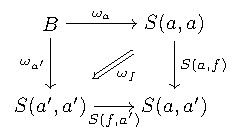
\includegraphics[scale=1]{figures/fig14}
\end{center}
A long and straightforward unwinding of universal properties shows that the category $\C/\!\!/c$ enjoys the universal property of the lax colimit $q\underrightarrow{\dashlim}\C(\firstblank,c)$.
\end{example}
\begin{remark}[The twisted arrow category as a lax colimit]
This is an interesting remark. It is possible to characterize the (opposite of the) twisted arrow category of \adef\refbf{twisted} as the lax colimit of the diagram $a\mapsto \A/a$, \ie as the lax coend
\[
\twoint^a \A/a.
\]
This is another long and straightforward exercise in unwinding universal properties, in a similar vein than Example \refbf{elts-as-coend}, that we leave to the interested reader.
\end{remark}
\begin{proposition}\label{lax.is.wcolim}
\cite[\S\textbf{2}]{bozapalides1980some} There is a canonical isomorphism between the lax end of a 2-functor $T\colon \C^\opp\times \C\to \B$ and the limit of $T$ weighted by the bifunctor $\C((\firstblank)^\diesis,\secondblank)$, \ie
\[
\wlim{\C((\firstblank)^\diesis,\secondblank)}T \cong \twoint_a T(a,a)
\]
where $\C((\firstblank)^\diesis,\secondblank)\colon (c, c')\mapsto \C(\firstblank,c')^\diesis(c)= \twoint^a \C(c,a)\times \C(a, c')$ is the \emph{lax composition} of relators. A dual statement holds for lax coends.
\end{proposition}
\begin{proof}
The classical argument which exploits the conservativity of the Yoneda embedding applies: we can compute
\begin{align*}
\B\left( b, \wlim{\C((\firstblank)^\diesis,\secondblank)}T \right) & \overset{(\refbf{homcommuteswei})}{=} \wlim{\C((\firstblank)^\diesis,\secondblank)} \B(b, T) \\
(\refbf{wlimcoends}) & \cong \int_{c,d} \B(b, T(c,d))^{\C(c^\diesis,d)}\\
& = \int_{c,d} \B(b, T(c,d))^{\twoint^a \C(c,a)\times \C(a, d)} \\ 
& \cong \twoint_a \int_{c,d} \left(\B(b, T(c,d))^{\C(a,d)} \right)^{\C(c,a)} \\
(\refbf{laxfubini})& \cong  \twoint_a \int_c \Cat\left( \C(c,a), \int_d \B(b, T(c,d))^{\C(a,d)} \right)\\
& \cong \twoint_a \int_c \Cat\left( \C(c,a), \B(b, T(c,a)) \right) \\
& \cong \twoint_a \B(b, T(a,a)) = \B\left(b, \twoint_a T(a,a)\right).\qedhere
\end{align*}
\end{proof}
We can define the \emph{tensor} of a category $\cate{T}$ with an object $a\in\A$, denoted $\cate{T}\cdot a$ by means of a lax coend; it is characterized by the natural isomorphism (in $x$)
\[
\Cat(\cate{T}, \A(a, x))\cong \A(\cate{T}\cdot a, x).
\]
Now, let $S\colon \A^\opp\to \Cat$, $T\colon \A\to \B$ be two functors and suppose $\B$ has $\Cat$-tensors; then the lax coend of the 2-functor $\A^\opp\times \A\xto{S\times T} \Cat\times\B\xto{\cdot} \B$ is called $q$-\emph{tensor product} of $S$ and $T$, denoted
\[
S\otimes T =: \twoint^a Sa\cdot Ta.
\]
More fundamental and subtle results, like the reduction of co/ends to co/limits, and the preservation of co/ends by the hom functors, remain valid for lax co/ends: %the rest of the section is devoted to explicitly prove all the basic statements present in \cite{bozapalides1980some}:
\begin{theorem}
In a 2-category $\B$, lax co/ends exist provided that $\B$ has co/comma objects and $\bf Cat$-co/limits.
\end{theorem}
\begin{theorem}
The lax end of the functor $T\colon \A^\opp\times \A \to \B$, if it exists, is uniquely determined by the natural isomorphism
\[
\B\left(x, \twoint_a T(a,a)\right)\cong \twoint_a \B(x, T(a,a))
\]
for every object $x\in \A$. A dual statement holds for lax coends.
\end{theorem}
\subsubsection{\bf Applications: $2$-distributors and lax Kan extensions.} A \emph{2-distributor} $\varphi \colon \A\leadsto \B$ is a 2-functor $\varphi\colon \B^\opp\times \A\to \Cat$. lax coends gives a method to compose 2-distributors, as in the 1-dimensional case: more precisely, let
\[
\A \overset{\varphi}{\leadsto}\B \overset{\psi}{\leadsto} \C
\]
be a couple of composable 2-distributors, namely two 2-functors $\varphi\colon \B^\opp\times \A\to \Cat$ and $\psi\colon \C^\opp\times \B\to \Cat$; then the composition $\psi\diamond \varphi$ is defined by the coend
\[
\psi\diamond \varphi(c,a) = \twoint^b \varphi(b,a)\times \psi(c,b)
\]
The compatibility between lax colimits and products ensures that the expected associativity holds up to a canonical identification:
\[
(\omega \diamond \psi)\diamond\varphi \cong \omega \diamond (\psi\diamond \varphi)
\]
for any three $\A\overset{\varphi}\leadsto\B\overset{\psi}\leadsto\C\overset{\omega}\leadsto\D$.

Let $T\colon \A\to \B$ and $\varphi\colon \A\to \C$ be two 2-functors.
\begin{definition}
We call \emph{(left) quasi-Kan extension} of $\varphi$ along $T$ a 2-functor $\Lan_T\varphi\colon \B\to \C$ endowed with a quasi-natural transformation $a\colon \varphi \Rightarrow \Lan_T\varphi\circ T$ (a \emph{unit}) such that, for each 2-functor $S\colon \B\to \C$ endowed with $\lambda \colon \varphi \Rightarrow S\circ T$ there exists a unique $\Cat$-natural transformation $\zeta\colon \Lan_T\varphi \Rightarrow S$ such that 
\[
(\zeta * T)\circ \alpha = \lambda 
\]
and moreover, if $\Sigma\colon \lambda \Rrightarrow \lambda'$ is a modification between quasi-natural transformations, there is a unique modification $\Omega\colon \zeta\Rrightarrow \zeta'$ (where $\zeta$ is induced by $\lambda$, and $\zeta'$ by $\lambda'$) between $\Cat$-natural transformations such that $(\Omega * T)\circ \alpha = \Sigma$. This can be expressed with the isomorphism
\[
\Fun(\A, \C)\Big[ \varphi, S\circ T \Big]\cong \C^{\B}\Big[ \Lan_T\varphi, S \Big]
\]
which is natural in $S$.
\end{definition}
\begin{example}
The quasi-Kan extension of a 2-functor $\varphi\colon \A\to\C$ along the trivial 2-functor $\A\to \cate{1}$ is the lax colimit of $\varphi$.
\end{example}
\begin{remark}
We can obtain different notions of quasi-Kan extension by reversing the directions of $\alpha, \lambda, \zeta$ etc.

The example above, as well as the following theorem, shows that the choice of $\Cat$-natural transformations instead of quasi-natural transformations is the right choice (see also \cite{bozapalides1980some} for a dual statement):
\end{remark}
\begin{theorem}\label{pseudolan}
Notations as above. If $\C$ has at least tensors $\B(Ta, b)\cdot \varphi a'$ for each $a, a'\in \A$, and the lax coends
\[
\twoint^a \B(Ta, b)\cdot \varphi a
\]
then the quasi-Kan extension of $\varphi$ along $T$ exists, and it is given by the formula above.
\end{theorem}
We can mimick also Exercise \textbf{2}.\refbf{closed.via.coends} to obtain a lax analogue of it:
\begin{proposition}
Let $\LNat(U,V)$ denote the category of lax natural transformations between two 2-functors $U,V$. Then
\[
\LNat(F\times G,H)\cong \LNat(F, H^G),
\]
where $H^G(x) = \LNat(\yon(A)\times G, H) = \twoint_y\Set(\hom(y,x)\times Gy, Hy)$
\end{proposition}
\begin{proof}
It is a computation in coend-fu, and every step can be motivated by results in the present section: calculemus.
\begin{align*}
\LNat(F, H^G) &= \twoint_x \Sets(Fx, \LNat(\yon(A)\times G, H))\\
&\cong \twoint_x \twoint_y \Sets(Fx, \Set(\hom(y,x)\times Gy, Hy))\\
&\cong \twoint_y\Set\Big(\Big(\twoint^x Fx \times \hom(y,x)\Big)\times Gy, Hy \Big)\\
&\cong  \twoint_y\Set\big( Fy\times Gy, Hy \big)\\
&=\LNat(F\times G,H).\qedhere
\end{align*}
\end{proof}
\subsection{Homotopy coends and $\infty$-coends.}
Higher category theory is now living a Renaissance, thanks to a massive collaboration of several people drawing from various fields of research, and cooperating to re-analyze every feature of category theory in the topos of simplicial sets.

Several reasons, and the urge to keep this chapter finite-dimensional force us to take for granted a certain acquaintance with the language of $\infty$-categories \emph{à la} Joyal-Lurie, but we also try to offer at least an intuition for what's going on and why things are done that way. The reader seeking a deeper understanding of this topic is advised to quit their job and move to Mojave desert with \cite{HTT,Joy,Joyal2002,JoyS} and a bag full of good weed.

Here we present the theory of \emph{homotopy co/ends} in model category theory, and then we move to the theory of \emph{simplicially coherent} and \emph{quasicategorical} co/end calculus. A final paragraph explores the definition of a co/end in a \emph{derivator}, and this  concludes the discussion of co/end calculus in each of the most common models for higher categories (model categories, enriched categories, simplicial sets, derivators). We leave aside a rather important question, that is \emph{model dependence}: for example, does an homotopy co/end correspond to an $\infty$-co/end if we pass from model categories to quasicategories?

In our discussion we follow the unique references available: \cite{Isaacson} for co/ends in model categories, \cite{cordier1997homotopy} for $\sSet$-enriched co/ends, and \cite{gepner2015lax} for quasicategorical ones. The definition of a coend in a derivator comes from the extensive treatment of category theory in Grothendieck's derivators started by M\@. Groth \cite{groth2013derivators}.
\subsubsection{\bf Co/ends in model categories.}\label{coends-in-model}
One of the most important parts of model category theory (the study of those structures that set homotopy theory in a purely formal framework) is the study of homotopy co/limits.

It is a fact, inherent to the theory, that colimit functors $\varinjlim_{\cate J}\colon \C^\cate{J}\to \C$are often quite ill-behaved with respect to a homotopical structure: such a thing is determined by the specification of a distinguished class of arrows $\mathcal W\subseteq \hom(\C)$ (these are called \emph{weak equivalences}) which is the class of isomorphisms in a ``localization'' of $\C$. If $\C$ has such a structure, then every category $\C^{\cate{J}}$ acquires an analogous structure $\mathcal{W}^\cate{J}$ where $\eta\colon F\Rightarrow G$ is in $\mathcal{W}^\cate{J}$ if and only if each component $\eta_j\colon Fj\to Gj$ is in $\mathcal W$. 

It is a fact that the image of such a natural transformation $\eta\colon F\Rightarrow G$ under the colimit functor, $\varinjlim\eta\colon \varinjlim F\to \varinjlim G$ is not always a weak equivalence.\footnote{A minimal instructive example goes as follows: take $\cate J$ to be the generic span $1\leftarrow 0\to 2$ and the functor sending it to $* \leftarrow S^{n-1}\to *$; the colimit of $F$ is the terminal space $*$. We can replace $F$ with the diagram $D^2 \leftarrow S^{n-1}\to D^2$, and since disks are contractible there is a homotopy equivalence $\tilde F \Rightarrow F$; unfortunately, the induced arrow $\varinjlim \tilde F = S^2\to *$ is not a weak equivalence.}

This is an unavoidable feature of the colimit functor $\varinjlim_{\cate J}\colon \C^\cate{J}\to \C$. One of the main tenets of homotopy theory is, nevertheless, that it doesn't matter if we replace an object with another, as soon as the two yield equivalent results. There is hope, then, that the \emph{category} of functors $\C^\cate{J}$ contains a better-behaved representative for the functor $\varinjlim$, and that the two are linked by some sort of weak- or homotopy equivalence.

That's what a homotopy colimit is: a deformation $\hocolim$ of $\varinjlim$ that preserves pointwise weak equivalences. And this is a general procedure in homotopy theory, where most objects $X$ are not ``compatible'' with the homotopical structures we superimpose on our category of spaces, and yet one is often able to find better-behaved representatives $\tilde X$ in the same homotopy class.

This said, there are mainly two ways to link co/end calculus and homotopy theory:
\begin{itemize}
\item In nice situations, homotopy co/limits can be computed as co/ends: the first attempt to clarify this construction was given in \cite{MR0365573}; nice explanatory surveys about this theory (touching also homological algebra) are \cite{hormann2014homotopy} and \cite{Gamb}.% This has already been discussed in Example \refbf{hocolimses}
\item The co/end functor $\int\colon \Cat(\C^\opp\times\C,\D)\to \D$ (as a particular colimit) can be ``derived'' yielding an \emph{homotopy co/end} functor $\int\colon \Cat(\C^\opp\times\C,\D)\to \D$ that preserves weak equivalences. This perspective, which is not independent from \cite{cordier1997homotopy}'s point of view, is expanded in \cite{DrorFar98} and \cite{Isaacson}.
\end{itemize}
These are respectively a co/end calculus \emph{applied to} model categories and \emph{interpreted in} model categories. The interplay and mutual completion of these two perspectives is evident.
% \begin{theorem}[The duality between two formulas for homotopy colimit]

% \end{theorem}
% \begin{remark}
% The real content of \cite{Gamb}
% \end{remark}
\begin{remark}
Let $\boxtimes \colon \A \times \B \to \C$ be the \textsc{t} part of a \textsc{thc} situation (see \refbf{tiaccaci}), which is moreover left Quillen, and let $\mathcal{I}$ be a Reedy category (\cite[\adef\textbf{5.2.1}]{Hov}). Then the coend functor
\[
\int \colon \Cat(\mathcal{I}^\opp,\A) \times \Cat(\mathcal{I},\B) \to \C
\]
is a left Quillen bifunctor if we regard the functor categories $\Cat(\mathcal{I}^\opp,\A)$ and $\Cat(\mathcal{I},\B)$ endowed with the Reedy model structure. The same is true if $\mathcal{I}$ is not Reedy, but the categories $\A,\B,\C$ are all combinatorial, and there is the projective model structure on $\Cat(\mathcal{I},\B)$, and the injective on $\Cat(\mathcal{I}^\opp,\A)$.
\end{remark}
% \begin{remark}
% A second linking result: the co/bar construction.
% \end{remark}
% \begin{definition}
% The derivator $Ho(\C^{\firstblank})$;
% \end{definition}
% \begin{definition}
% Homotopy co/end functor.
% \end{definition}
% \begin{example}

% \end{example}
% \begin{proposition}

% \end{proposition}
% \trans{TO BE WRITTEN.}
\subsubsection{\bf Co/ends in quasicategories.}
\begin{remark}
As a rule of thumb, the translation procedure from category to $\infty$-category theory is based on the following meta-principle: first you rephrase the old definition in a ``simplicially meaningful'' way, so that the $\infty$-categorical definition specializes to the old one for quasicategories $N(\C)$ which arise as nerves of categories. Then you forget about the original gadget and keep the simplicial one; this turns out to be the right definition. 

The first victim of this procedure is the twisted arrow category \refbf{twisted} of an $\infty$-category.
\end{remark}
\begin{definition}[Twisted arrow $\infty$-category]
Let $\varepsilon\colon \bDelta\to \bDelta$ be the functor $[n]\mapsto [n]\star [n]^\opp$, where $\star$ is the join of simplicial sets \cite{Joy,ehlers2008ordinal}. Let $\C$ be a $\infty$-category; the twisted arrow category $\tw(\C)$ is defined to be the simplicial set $\varepsilon^*\C$, where $\varepsilon^*\colon \sSet \to \sSet$ is the induced functor. More explicitly, and consequently, the $n$-simplices of $\tw(\C)$ are characterized by the relation
\[
\tw(\C)_n \cong \sSet(\Delta[n], \tw(\C))\cong \sSet(\Delta[n]\star \Delta[n]^\opp, \C).
\]
\end{definition}
The most important feature of the twisted arrow category is that it admits a fibration over $\C^\opp\times\C$ (part of its essential properties can be deduced from this); the machinery of left and right fibrations exposed in \cite[\adef\textbf{2.0.0.3}]{HTT} gives that 
\begin{itemize}
\item There is a canonical simplicial map $\Sigma\colon \tw(\C) \to \C^\opp\times\C$ (induced by the two join inclusions $\Delta[\firstblank], \Delta[\firstblank]^\opp \to \Delta[\firstblank]\star \Delta[\firstblank]^\opp$);
\item This $\infty$-functor is a right fibration in the sense of \cite[\adef\textbf{2.0.0.3}]{HTT}.
\end{itemize}
\begin{remark}
It is rather easy to see that the above definition is reasonable: a 0-simplex in $\tw(\C)$ is an edge $f \colon \Delta[1]\to \C$, and a 1-simplex of $\tw(\C)$ is a 3-simplex thereof, that we can depict as a pair of edges $(u,v)$, such that the square having twisted edges
\[
\xymatrix{
	\ar[d]_f & \ar[l]_u \ar[d]^{f'}\\
	\ar[r]_v &
}
\]
commutes. This suggest (as it must be) that the definition of $\tw(\C)$ for a $\infty$-category specializes to the 1-dimensional one and adds higher-dimensional informations to it.
\end{remark}
\begin{definition}\label{infend}
Let $\C,\D$ be two $\infty$-categories; the \emph{co}/\emph{end} of a simplicial map $F\colon \C^\opp\times \C\to \D$ is the co/limit of the composition 
\[
\tw(\C)\xto{\Sigma} \C^\opp\times \C \xto{F} \D
\]
\end{definition}
The main interest of the authors in \cite{gepner2015lax} is to formulate an analogue of \refbf{fibelem}, which characterizes the Grothendieck construction of a $\Cat$-valued functor as a particular weighted colimit (see \refbf{elts-as-coend}).

It is rather easy to formulate such an analogue definition: this appears as \cite[\adef \textbf{2.8}]{gepner2015lax}.
\begin{definition}[op/lax colimit of $F$]
Let $F\colon \C\to \Cat_\infty$ be a functor between $\infty$-categories. We define
\begin{itemize}
\item the \emph{slice fibration} for $\C \in\cate{QCat}$ to be the functor of quasicategories $\chi_\C \colon \C \to \cate{QCat}$ sending $c\in\C$ to $\C_{/c}$, and dually the \emph{coslice fibration} to be $\chi^\C \colon \C \to \cate{QCat} \colon c \mapsto \C_{c/}$;
\item the \emph{lax colimit} of $F$ to be the coend
\[
\infint^c \C_{c/}\times Fc;
\]
\item the \emph{oplax colimit} of $F$ to be the coend
\[
\infint^c \C_{/c}\times Fc.
\]
\end{itemize}
\end{definition}
The Grothendieck construction associated to $F$, discussed in \cite{HTT} with the formalism of un/straightening functors results precisely as the oplax colimit of $F$. This is coherent with our \refbf{elts-as-coend} and \refbf{its.another.nerve}.
\subsection{Simplicially coherent co/ends.}
All the material in the following subsection comes from \cite{cordier1997homotopy}. Since we are forced to divert from \cite{cordier1997homotopy}'s notation by our personal choices and a slight pedantry, we begin the exposition establishing a convenient notation and a series of useful short-hands. We decided to keep this introduction equally self-contained and simple, but we can't help but admit that
\begin{itemize}
\item there is a sheer amount of (unavoidable, and yet annoying) sins of omissions in this survey section, basically due to the ignorance of the author; moreover, the price to pay to obtain a self-contained exposition is to deliberately ignore several subtleties, exposing  the theory to a certain na\"ivety.
\item there are newer and more systematic approaches to this topic, owing a great debt to \cite{cordier1997homotopy} but capable to generalize sensibly their constructions; among many, the reader should consult the exceptionally clear \cite{riehl2014categorical,shulman}. All these references reduce the construction of a simplicially coherent co/end to the ``unreasonably effective'' co/bar construction \cite[\achap\textbf{4}]{riehl2014categorical}: this is not the case, as it can be proved \cite[21.4]{shulman} that the coherent co/end of $T$ results as a suitable \emph{derived weighted co/limit} of the functor $T$.
\end{itemize} 
It is our sincere hope that this does not affect the outreach of this elegant and neglected piece of Mathematics, and the clumsy attempt to popularize an account of \cite{cordier1997homotopy} has to be seen as an attempt to communicate how beautiful we find this writing, as it is (one of) the beginner(s) of \emph{categorical homotopy theory}.
\paragraph{\bf Local notation.} All categories $\A,\B,\dots$ appearing in this subsection are enriched over $\sSet = [\bDelta^\opp , \Set]$. All of them possess the co/tensors (see \adef\refbf{tenscotens}) needed to state definitions and perform computations. These functors assemble into a \textsc{thc} situation (see Remark \refbf{tiaccaci}) $\tee = (\cdot, \hom, \pitchfork)$ where $\cdot \colon \sSet \times \A \to \B$ determines the variance of the other two functors. A useful shorthand to denote the functor $\pitchfork(K,A) = K \pitchfork A$ (especially when it is necessary to save space or invoke the ``exponential'' behaviour of this operation) is $A^K$. We switch rather freely among these two notations.
\begin{definition}[Totalization]
Let $Y^\bullet \colon \bDelta^\opp \times \bDelta \to \B$ be a simplicial-cosimplicial object; we define the \emph{totalization} $\textsf{tot}(Y^\bullet_\bullet)$ of $Y^\bullet$ to be the end
\[
\Big(\int_{n\in\bDelta} \Delta[n]\pitchfork Y^n\Big)^\bullet
\]
(it is a cosimplicial object). The totalization of $Y^\bullet$ is also denoted with the shorthand $\bDelta^\bullet\pitchfork Y^\bullet$ or similar.
\end{definition}
\begin{definition}[Diagonalization]
Let $X_\bullet \colon \bDelta^\opp\times \bDelta^\opp \to \B$ be a bisimplicial object; we define the \emph{diagonalization} $\textsf{diag}(X_\bullet)$ of $X_\bullet$ to be the coend
\[
\Big(\int^{n\in\bDelta} \Delta[n]\cdot X_n\Big)_\bullet
\]
(it is a simplicial object) The diagonalization of $X_\bullet$ is also denoted with the shorthand $\bDelta^\bullet \cdot X_\bullet$ or similar.
\end{definition}
\begin{notat}[Chain co/product]
Let $\A \in \sSet\text{-}\Cat$, and $\vec x_n = (x_0,\dots, x_n)$ the ``generic $n$-tuple of objects'' in $\A$; given additional objects $a,b\in\A$ define a bisimplicial set $\amalg\A[a| \vec x | b]_\bullet$ whose simplicial set of $n$-simplices is
\[
\amalg\A[a| \vec x_n | b]_\bullet := 
\coprod_{x_0,\dots, x_n \in \A} 
\A(a,x_0)_\bullet\times \A(x_0, x_1)_\bullet \times \cdots \times \A(x_n,b)_\bullet.
\footnote{It is useful to extend this notation in a straightforward way: $\A[a|\vec x | b]$ denotes the product $\A(a,x_0)\times \A(x_0, x_1) \times \cdots \times \A(x_n,b)$, and $\Pi \A[a|\vec x|b]$, $\A[\vec x]$, $\Pi \A[\vec x]$, $\amalg \A[\vec x]$ are defined similarly. Note that $\amalg\A[a| \vec x_n | b]_\bullet$ does not depend on $\vec x_n$ since the coproduct is quantified over all such $\vec x_n$'s.}
\] 
Faces and degeneracies are induced, respectively, by composition and identity-insertion (see Exercise \textbf{7}.\refbf{ex8:Y-of-T}).

Finally we define the simplicial set $\delta\A(a,b)$ to be $\diag (\amalg\A[a|\vec x_\bullet|b]_\bullet) = n\mapsto \amalg\A[a|\vec x_n|b]_n$. Couched as a coend, $\delta\A(a,b)$ is written
\begin{align*}
\delta\A(a,b) &\cong \int^{n\in\bDelta} \Delta[n]\times \amalg\A[a| \vec x_n | b] \\
&= \int^{n\in\bDelta} \Delta[n]\times \coprod_{x_0,\dots, x_n \in \A} \A(a,x_0)\times \A(x_0, x_1) \times \cdots \times \A(x_n,b)\\
&\cong \int^{n\in\bDelta} \coprod_{x_0,\dots, x_n \in \A} \Delta[n]\times \A(a,x_0)\times \A(x_0, x_1) \times \cdots \times \A(x_n,b)
\end{align*}
\end{notat}
\begin{definition}[The functors $\Y$ and $\W$]
Let $T \colon \A^\opp\times \A \to \B$ be a functor; we define $\Y(T)^\bullet$ to be the cosimplicial object (in $\B$)
\[
\Y(T)^n := \prod_{\vec x = (x_0,\dots, x_n)} \A[\vec x_n]\pitchfork T(x_0, x_n)
\] 
where $\A[\vec x_n] = \A(x_,x_1) \times \dots \times \A(x_{n-1},x_n)$.
Dually, given the same $T$, we define $\W(T)_n$ to be the simplicial object (in $\B$)
\[
\W(T)_n := \coprod_{\vec x = (x_0,\dots, x_n)} \A[\vec x_n] \cdot T(x_0, x_n).
\]
\end{definition}
\begin{example}
If we consider $\A$ to be trivially enriched (or as someone says, a \emph{discrete} simplicial category), then the object $\A[a|\vec x_n|b]_\bullet$ coincides with the nerve of the category $(a\downarrow \A \downarrow b)$ of arrows ``under $a$ and above $b$''.
\end{example}
\begin{definition}[Simplicially coherent co/end]\label{cohcoend}
Let $T \colon \A^\opp\times \A \to \B$ be a functor. We define
\begin{gather}
\small
\oint_a T(a,a) := \int_{a',a''} T(a',a'')^{\delta \A(a', a'')} \quad
\oint^a T(a,a) := \int^{a',a''}\delta \A(a',a'') \cdot T(a',a'')
\end{gather}
to be the \emph{simplicially coherent co/end} of $T$.
\end{definition}
In a few words, the definition of a $\sSet$-coherent co/end involves the classical construction but adds to the scene ``fattened up'' co/tensors $\A[a|\vec x|b]$ and suchlike, organized as a functor $ \A^\opp\times \A \times \A^\opp\times \A \to \B$ in such a way that the co/end is on two variables $a',a'' \in \A$.
\begin{remark}[\righteyes, coherent co/ends as deformations]
Example \refbf{ends-are-weighted} gives that co/end are weighted co/limits, and precisely weighted co/limits with the $\hom$ weight. This perspective is useful here, since we write that $\oint_a T$ is the end $\int_{(a',a'')\in \A^\opp\times \A} T(a',a'')^{\hom(a',a'')}$ where we applied a suitable ``deformation'' (or ``resolution'', or ``replacement'') functor $\delta$ to the hom functor $\A(\firstblank,\secondblank)$, seen as the identity relator (Remark \refbf{profundefs}). To some extent this point of view is explored in \cite{nashphd} in the particular case where $\V\text{-}\Cat = \textsc{dg}\text{-}\Cat$; we have taken something from, as well as given something to, that document. 

This perspective is of great importance to encompass coherent co/ends into a general theory ``compatible'' with some model structure on $\VCat$, for some monoidal model $\V$ and the Bousfield-Kan model structure on $\VCat$. Expanding this point of view, will be, hopefully, the subject of \cite{inftycoends}.
\end{remark}

\paragraph{\bf Homotopy coherent calculus}
Classical co/end calculus (in the triptych Fubini - Yoneda - Kan) is an invaluable tool (in fact, the only and most natural one) to prove several results even in the simplicial setting: as it is customary in the salons of higher category theory, we will always reduce a computation involving a coherent, and yet indirectly defined object, to a computation involving a ``concrete'', and yet complicated object which takes into account the coherence introduced in the deformation.

\cite{cordier1997homotopy} succeed in the indeed quite ambitious task to to rewrite \emph{all} the most important pieces of classical category theory in this ``higher'' model (the paper contains a calculus for co/limits, mapping spaces, Yoneda, and Kan extensions). The aim of the rest of this subsection is to sketch some of these original definitions, hopefully helping an alternative formulation of $(\infty,1)$-category theory (the authors of whom we owe a great debt, were it only for having proved --in 1997!-- that the ``$\infty$-categorical dogma'' can be avoided\footnote{The subtle monophysism called ``$\infty$-categorical dogma'' asserts that `quasicategory' and `$\infty$\hyp{}category' are synonyms.}) to escape oblivion: we do not claim to give a complete account of this theory here, and instead address the interested reader to their beautiful original paper.
\begin{proposition}
Let $T\colon \A^\opp\times \A \to \B$ be a $\sSet$-functor. Then there is a canonical isomorphism
\[
\oint_a T(a,a) \cong \textsf{tot}(\Y(T)^\bullet)
\]
\end{proposition}
\begin{proof}
We use heavily the ninja Yoneda lemma \refbf{ninjayo} in its enriched form, where 
\[
\int_X \A(X,B) \pitchfork F(X) \cong F(B)
\]
and the fact that $K \pitchfork (H \pitchfork A)\cong (K\otimes H)\pitchfork A$, naturally in all arguments.

With this remark in hand we can move to the real proof: $\vec x = (x_0,\dots, x_n)$ is a generic tuples of objects of $\A$, and to save some space we switch to the notation $A^K$ to denote $K\pitchfork A$.
\begin{align*}
\oint_a T(a,a) &:= \int_{a',a''} T(a',a'')^{\delta\A(a',a'')}\\
&\cong \int_{a',a''}  		  T(a',a'')^{\int_n \Delta[n]\times \amalg \A[a'|\vec x| a'']}\\
&\cong \int_{a',a'',n}		  T(a',a'')^{\Delta[n]\times \amalg \A[a'|\vec x| a'']}\\
&\cong \int_{a',a'',n} \left( T(a',a'')^{\A(x_n,a'')} \right)^{\Delta[n]\times \amalg \A[a'|\vec x]}\\
&\cong \int_{a',a'',n} \prod_{x_0,\dots, x_n} \left( T(a',a'')^{\A(x_n,a'')} \right)^{\Delta[n]\times \A[a'|\vec x]}\\
&\cong \int_{a',n}     \prod_{x_0,\dots, x_n} \left( \int_{a''} T(a',a'')^{\A(x_n,a'')} \right)^{\Delta[n]\times \A[a'|\vec x]}\\
&\cong \int_{a',n}     \prod_{x_0,\dots, x_n} T(a',x_n)^{\Delta[n]\times \A[a'|\vec x]}\\
&\cong \int_{n}        \prod_{x_0,\dots, x_n} \left( \int_{a'} T(a',x_n)^{\A(a',x_0)} \right)^{\Delta[n]\times \A[\vec x]}\\
&\cong \int_{n}   \Big(\prod_{x_0,\dots, x_n} T(x_0,x_n)^{\A[\vec x_n]}\Big)^{\Delta[n]} \cong \textsf{tot}(\Y(T)).\qedhere
\end{align*}
\end{proof}
For the sake of completeness, we notice that the universal wedge testifying that $\oint_a T(a,a) \cong \textsf{tot}(\Y(T))$ is induced by the morphisms
\begin{center}
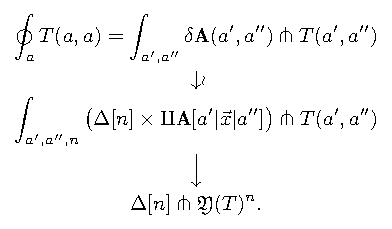
\includegraphics[scale=1]{figures/fig13}
\end{center}
Prove the dual statement as an exercise (to finish the proof it is of vital importance to exploit a good notation):
\begin{proposition}
Let $T\colon \A^\opp\times \A \to \B$ be a $\sSet$-functor. Then there is a canonical isomorphism
\[
\oint^a T(a,a) \cong \textsf{diag}(\W(T)_\bullet)
\]
\end{proposition}
\subsubsection{\bf Simplicially coherent natural transformations}
\begin{remark}
The homotopy coherent co/ends admit ``comparison'' maps to the classical co/ends; this is part of a general tenet of higher category theory, where homotopically correct objects result as a \emph{deformation} of classical ones, and this deformations maps into/out of the classical object.

The comparison map $\oint T(a,a) \to \int T(a,a)$ arises, here, as an homotopy equivalence between the simplicial set $\A(a,b)$ (seen as bisimplicial, and constant in one direction) and the bisimplicial set $\delta \A(a,b) = \diag \A[a|\bullet|b]_\bullet$: this is \cite[p. 15]{cordier1997homotopy}.

The map
\[
d_0 \colon \coprod_{x_0} \A(a, x_0)\times \A(x_0,b) \to \A(a,b)
\]
given by composition has an homotopy inverse given by
\[
s_{-1}\colon \A(a,b) \to \A(a, a)\times \A(a,b)\colon g\mapsto (\id_a, g).
\]
Indeed, the composition $d_0 s_{-1}$ is the identity on $\A(a,b)$, whereas the composition $s_{-1} d_0$ admits  is homotopic to the identity on $\delta \A(a,b)$ (we use the same name for the maps $d_0, s_{-1}$ and the induced   maps $\bar d_0 \colon \delta \A(a,b) \to \A(a,b)$, induced by the universal property, and $\bar s_{-1}\colon \A(a,b) \to \delta \A(a,b)$).

There is an important difference between these two maps, though: whilst $d_0$ is natural in both arguments, $s_1$ is natural in $B$ but not in $A$. This has an immediate drawback: whilst $d_0$ can be obtained canonically, as the universal arrow associated to a certain natural isomorphism (see (\refbf{dizzero}) below), $s_{-1}$ can't (the best we can do is to characterize the natural argument of $s_{-1}$ via \cite[Example \textbf{2}, p. 16]{cordier1997homotopy}).
\end{remark}
As we have seen in \refbf{naturalu}, the set of natural transformations between two functors $F,G \colon \C \to \D$ coincides with the end $\int_x \D(Fx, Gx)$, and (see \refbf{laxnat}) the category of lax natural transformations between two 2-functors coincides with the lax end $\sqint_x \D(Fx, Gx)$. It comes as no surprise, then, that the following characterization of \emph{homotopy coherent} natural transformations between two simplicial functors hold:
\begin{definition}[Coherent natural transformations]
Let $F,G \colon \C \to \D$ be two simplicial functors; then the simplicial set of \emph{coherent transformations} between $F$ and $G$ is defined to be
\[
\textsf{Coh}(F,G) := \oint_a \D(Fa, Ga).
\]
\end{definition}
\def\opitchfork{\mathop{\overline{\pitchfork}}}
\def\uotimes{\mathop{\underline{\otimes}}}
\begin{definition}[Mean tensor and cotensor]
Let $F \colon \A \to \B$, $G\colon \A \to \sSet$, $H\colon \A^\opp \to \sSet$.
We define $G \opitchfork F$, $H \uotimes F$ respectively as 
\[
G \opitchfork F := \oint_a Ga\pitchfork Fa \qquad\qquad 
H \uotimes F := \oint^a Ha \otimes Fa.
\]
\end{definition}
\begin{definition}[Standard resolutions]
Let $F\colon \A \to \B$ be a simplicial functor; we define
\begin{align*}
\overline{F}a &:= \A(a,\firstblank)\opitchfork F = \oint_x \A(a,x)\pitchfork Fx\\
\underline{F}a &:= \A(\firstblank,a)\uotimes F =  \oint^x \A(x,a)\otimes Fx.
\end{align*}
\end{definition}
\begin{example}\label{thehoms}
We specialize the above definition to compute the functors
$\overline{\hom}(a,\firstblank)$ and $\underline{\hom}(a,\firstblank)$: in particular we concentrate on the second case, since the first is completely dual. Calculemus:
\begin{align*}
\underline{\hom}(a,b) & = \oint^a \A(a,x) \times \A(x,b)\\
&\cong \int^{xy} \delta \A(x,y) \times \A(a,x)\times \A(y,b)\\
&\cong \int^{xy} \A(a,x)\times \delta\A(x,y) \times \A(y,b)\\
&\cong \int^{xyn} \coprod_{x_0,\dots, x_n} \A(a,x)\times \A(x,x_0)\times \dots\times \A(x_n,y)\times \A(y,b)\times \Delta[n]\\
&\cong \int^{xyn} \A[a|\tilde{x}_n|b]\times\Delta[n] \cong \delta \A(a,b).
\end{align*} 
\end{example}
We leave as an easy exercise in co/end-fu the proof of the following result (see Exercise \refbf{ex8:cohnat}), which shows that the standard resolutions $\underline{(\firstblank)}, \overline{(\firstblank)}$ `absorb the coherence informations':
\begin{proposition}\label{absorb}
Let $F,G \colon \C \to \D$ be two simplicial functors; then there are canonical isomorphisms 
\[
\Nat(F, \overline G) \cong \textsf{Coh}(F,G) \cong \Nat(\underline F,G).
\]
\end{proposition}
This result has a number of pleasant consequences: the simplicially coherent setting is powerful enough to retrieve several classical constructions.
\begin{itemize}
\item Example \refbf{thehoms} above shows that $\underline{\hom}(a,\firstblank)(b)\cong \delta \A(a,b)$; this entails that there is an isomorphism
\[\label{dizzero}
\Nat(\delta \A(a,\firstblank), \A(a, \secondblank)) \cong
\textsf{Coh}(\A(a,\firstblank),\A(a,\secondblank))
\]
and it is a matter of verifying some additional nonsense to see that the $\sSet$-natural transformation corresponding to the identity coherent transformation is precisely $d_0$.
\item The map $d_0$ defines additional universal maps $\eta_F , \eta^F$ which ``resolve'' a functor $F \colon \A \to \B$ whenever $\underline{F}, \overline{F}$ exist (it is sufficient that $\B$ admits all the relevant co/limits to perform the construction of $\underline{F}, \overline{F}$). From the chain of isomorphisms
\begin{align*}
\eta^F : \overline{F}b & = \oint_a \A(b,a)\pitchfork Fa\\
&\cong \int_{a',a''} \delta\A(a',a'')\pitchfork\A(b,a'')\pitchfork Fa'\\
&\leftarrow \int_{a',a''} \A(a',a'')\pitchfork\A(b,a'')\pitchfork Fa'\\
(\refbf{ninjayo}) &\cong Fb;\\
\eta_F : \underline{F}b &= \oint^a Fa \otimes \A(a,b)\\
&\cong \int^{a',a''} Fa' \otimes \A(a'',b)\delta\A(a',a'')\\
&\to \int^{a',a''} Fa' \otimes \A(a'',b)\A(a',a'')\\
&\cong Fb;
\end{align*}
we obtain  natural transformations corresponding to suitable coherent identities under the isomorphism of \aprop\refbf{absorb}.
\item The maps $\eta_F , \eta^F$ behave like resolutions: \cite[\aprop\textbf{3.4}]{cordier1997homotopy} shows that they are level-wise homotopy equivalences (meaning that $\eta_F \colon Fa \to \overline{F}a$ induces homotopy equivalences of simplicial sets $\B(b, Fa)\xto{(\eta_F)_*} \B(b, \overline{F}a)$ for each $b$, naturally in $b$).\footnote{We decide to skip the proof of this proposition, as it is quite long, technical, and even though it relies on co/end-fu it doesn't add much to the present discussion.}
\end{itemize}
% \begin{proposition}[The coherent Yoneda lemma]
% \todo[inline]{fare}
% \end{proposition}
\subsubsection{\bf Simplicially coherent Kan extensions}
The universal property characterizing a Kan extension is inherently 2-dimensional: uniqueness is stated at the level of 2-cells, and any sensible generalization of it to the higher world involves a ``space'' of 2-cells between 1-cells. This entails that any reasonable definition of a (left or right) Kan extension ultimately relies on a nice definition for a space of coherent natural transformations between functors, which has been the subject of the previous subsection. There are, nevertheless, several subtleties as there are many choices available for a definition: in the words of \cite{cordier1997homotopy},
\begin{quote}
Clearly one can replace $\Nat$ by $\textsf{Coh}$ [in the definition of a Kan extension], but should isomorphism be replaced by homotopy equivalence, should this be natural, in which direction should this go\dots ?
\end{quote}
As it turns out from \cite{cordier1997homotopy}, the right way to preserve a reasonably vast calculus for Kan extensions is to ask that the isomorphisms
\begin{gather*}
\Nat(H,\hoRan_G K)\cong \textsf{Coh}(HG,K)\\
\Nat(\hoLan_G H,K)\cong \textsf{Coh}(H,KG)
\end{gather*}
hold. This can be achieved defining the left and right Kan extensions as follows:
\begin{definition}[Coherent Kan extensions]\label{cohkan}
Let $F \colon\A \to \C$ and $G\colon \A \to \B$ be a span of simplicial functors; we define
\begin{gather*}
\hoRan_G F(\firstblank) = \oint_a \B(\firstblank,Ga)\pitchfork Fa\\
\hoLan_G F (\firstblank) = \oint^a \B(Ga,\firstblank)\otimes Fa
\end{gather*}
\end{definition}
\begin{remark}
This can be seen as a simplicially coherent analogue of our \refbf{pseudolan}; it is not a coincidence that lax and simplicially coherent co/end calculi mimick each other: 2-co/ends correspond to suitable ``truncated'' simplicially coherent co/ends (and this correspondence can be made functorial). 

In the same spirit of \cite{bozapalides1980some}, a co/endy view on categorical homotopy theory sheds a light on several geometric constructions (see \cite{cordier1997homotopy} for more informations and links with \cite{MR1080880,segal1974a}).
\end{remark}
We would like to prove, now, that the isomorphisms defining a Kan extension hold with the definitions above. This is a computation in co/end-fu, which at this point can be left as an exercise for the reader.
\subsubsection{\bf Co/ends in a derivator.}
The theory of derivators serves as a purely 2-categorical model for higher category theory, where all the coherence informations are encoded in coherence conditions for suitable diagrams of 2-cells. Here we only sketch some of the basic definitions needed to pave the way to \adef\refbf{coendinder} below.
\begin{definition}[The 2-category of prederivators]
A \emph{prederivator} is a strict 2-functor $\D\colon \Cat^\opp\to \cate{CAT}$ (where $\cate{CAT}$ is the category of $\mho^+$-categories, see the two-universe convention in the introduction); a \emph{morphism of prederivators} is a pseudonatural transformation between pseudofunctors, $\eta\colon \D\Rightarrow \D'$; a \emph{2-cell} between morphisms of prederivators is a modification (see \adef\refbf{modification}) $\Theta\colon \eta\Rrightarrow \eta'$ between pseudonatural transformations.

These data form the \emph{2-category of prederivators}.
\end{definition}
The notion of a \emph{derivator} arises as a refinement of this; apart from some minor (milder, but not less important) assumptions, a derivator is a prederivator $\D$ such that every $\D(u)\colon \D(J)\to \D(I)$, induced by $u\colon I\to J$ has both a left and a right adjoint, fitting into a triple
\[
u_!\dashv u^*\dashv u_*\colon\vcenter{\xymatrix@C=2cm{
	\D(J) \ar[r]|{u^*} & \ar@<-8pt>[l]_{u_*} \ar@<8pt>[l]^{u_!} \D(I)
}}
\]
(see \cite[\adef \textbf{1.10}]{groth2013derivators}). These functors are called respectively the \emph{homotopy left and right Kan extensions along $u\colon I\to J$}. Axiom (Der4) in \cite[\adef \textbf{1.10}]{groth2013derivators} states that these Kan extensions can always be computed with a \emph{pointwise} formula; this can be interpreted as a rephrasing of the theory exposed in our \textbf{2.1}, in view of the equivalence between all the following characterizations of $\Lan_G F(b)$/$\Ran_G F(b)$:
\begin{itemize}
\item the (right or left) Kan extension of $F\colon \A\to \C$ along $G\colon \A\to\B$ computed in $b$;
\item the weighted co/limit of $F$ with respect to the representable $\hom(G,b)$;
\item the conical co/limit of $F$ over the category of elements of $\hom(G,b)$;
\item the conical colimit of the diagram $(G\downarrow b)\to \A\xto{F}\B$.
\end{itemize}
Let $\textsc{Tw}(K)$ be the category of elements (\adef \refbf{eltsf}) of $\hom_K$, for a small category $K$; then there exists a functor $\Sigma_K = (t,s)\colon \textsc{Tw}(K)\to K^\opp\times K$ (\aprop \refbf{fibelem}). 
\begin{definition}[Homotopy coend in a derivator]\label{coendinder}
Let $\D$ be a derivator, and $K\in\Cat$ a category. The \emph{homotopy coend} $\int^K\colon \D(J\times K^\opp\times K)\to \D(J)$ is defined as the composition
\[\textstyle
\int^K\colon \D(J\times K^\opp\times K) \xto{\Sigma_K^*} \D(J\times \textsc{Tw}(K))\xto{\p_!} \D(J)
\]
\end{definition}
\begin{remark}
Let $\D(J|\firstblank)\colon \Cat^\opp \to \cate{CAT}$ be the \emph{shifted derivator} of $\D$, \ie the functor $I\overset{\firstblank\times J}\longmapsto I\times J \overset{\D(\firstblank)}\mapsto \D(I\times J)$. Then the coend $\int^K$ is a morphism between the shifted derivators $\D(K^\opp\times K|\firstblank)\to \D(\firstblank)$.
\end{remark}
\begin{remark}
There is obviously a similar notion of homotopy \emph{end} in $\D$: one only has to replace $\p_!$ with the right adjoint $\p_*$ in the definition above (taking the \emph{limit} over the twisted arrow category, instead of the colimit):
\[\textstyle 
\int_K  \colon \D(J\times K^\opp\times K) \xto{\Sigma_K^*} \D(J\times \textsc{Tw}(K))\xto{\p_*} \D(J)
\]
\end{remark}
\begin{lemma}
If $F\colon \D\to \D'$ is a morphism of derivators, there is a canonical ``comparison'' morphism
\[\textstyle 
\int^K \circ F \to F\circ \int^K
\]
obtained as the composition
\begin{center}
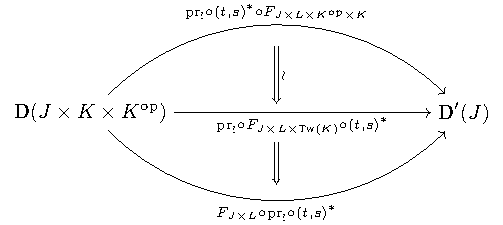
\includegraphics[scale=1]{figures/fig9}
\end{center}
where the second morphism results as the \textsc{bc} pasting
\[
\p_! F_J \xRightarrow{\p_! F_J \eta_{(\p_!\dashv \p^*)}}
\p_! F_J \p^*\p_! \xRightarrow{\p_! \varphi_J\p_!}
\p_! \p^* F_e\p_! \xRightarrow{\epsilon_{(\p_!\dashv \p^*)}F_e\p_!} Fe \p_!
\]
represented in the following diagram of 2-cells:
\begin{center}
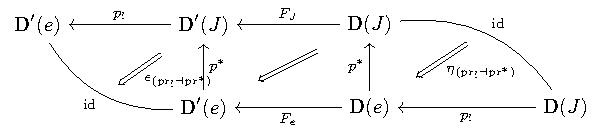
\includegraphics[scale=1]{figures/fig10}
\end{center}
\end{lemma}
It is almost a triviality that a derivator morphism $F$ \emph{preserves homotopy coends} (\ie the above 2-cell is invertible) if it preserves colimits, or more generally Kan extensions.
\begin{exerciseset}
\begin{exercisepoints}
\item \label{ex8:tw-as-a-laxlim} A \emph{lax colimit} for a diagram $F \colon \mathcal{J}\to \cate{K}$ in a 2-category $\cate{K}$ is an object $L$ with a \emph{lax cocone} $\{Fj \to L\}$ satisfying a suitable universal property (state it, mimicking --the dual of-- \adef\refbf{laxwedge}). Show that the opposite of the twisted arrow category $\tw(\C)$ of \adef\refbf{twisted} is the lax colimit of the diagram $\C \to \Cat \colon c \mapsto \C/c$ sending every object to its slice category.
\item \label{ex8:laxcoends} State the definition of lax \emph{cowedge} $S\xto{..}d$ for a 2-functor $S\colon \A^\opp\times \A\to \B$; state the definition of lax coend for $S$ as an \emph{initial} cowedge, the representing object of the functor $d\mapsto \textsf{LCwd}(S,d)$. 
\item \label{ex8:inserter} Show that $\textsf{Ist}(f,g)$ share the universal property of the $\Cat$-limit of the diagram $\{0\rightrightarrows 1\} \to \C$ choosing $f,g$ weighted by the $\Cat$-presheaf $\{0\rightrightarrows 1\} \to \Cat$ choosing the categories $\{0\} \underset{d_1}{\overset{d_0}\rightrightarrows} \{0<1\}$.
\item \label{ex8:Y-of-T} Define co/faces and co/degeneracies for the objects $\Y(T)$ and $\W(T)$ (hint: there is an isomorphism $\tau \colon T(x_0,x_n)^{\Pi \A[\vec x]}\cong \Big(T(x_0,x_n)^{\A(x_0,x_1)}\Big)^{\A[x_1|\vec y|x_n]_{n-1}}$, and you want to assemble a map $\Y(T)^{n-1}\to \Y(T)^n$ from its components $\Pi \A[\vec x] \pitchfork T(x_1,x_n) \to \Y(T)^n$; this defines $d^0$. The map $d^n$ is defined via an isomorphism $\sigma$ and a similar argument).
\item \label{ex8:cohfubini} Prove the Fubini theorem for simplicially coherent co/ends: given a functor $T\colon \A^\opp\times \A\times \B^\opp\times \B\to\C$, then
\[
\oint^a\left( \oint^b T(a,a,b,b)\right)\cong
\oint^{(a,b)\in\A\times\B} T(a,b,a,b)\cong
\oint^b\left( \oint^a T(a,a,b,b)\right)
\]
(it is a simple theorem about the relation between $\delta(\A\times\B)$ and $\delta\A\times\delta\B$!).
\item \label{ex8:cohnat} Prove that $\Nat(F, \overline G) \cong \textsf{Coh}(F,G) \cong \Nat(\underline F,G)$, using \adef \refbf{cohcoend} and a formal argument.
\item \label{ex8:cohkan} Prove that the isomorphisms
\begin{gather*}
\Nat(H,\hoRan_G K)\cong \textsf{Coh}(HG,K)\\
\Nat(\hoLan_G H,K)\cong \textsf{Coh}(H,KG)
\end{gather*}
hold defining coherent Kan extensions as in \refbf{cohkan}.
\item Prove that the standard resolutions ``absorb coherence'' in coherent Kan extensions, showing that
\[
\Ran_G \overline F \cong \hoRan_G F \qquad\qquad \Lan_G \underline F \cong \hoLan_G F .
\]
(a preliminary lemma: prove that $\overline F(\firstblank)\cong \int_a Fa^{\delta\A(\firstblank,a)}$).% and $\underline F (\firstblank) \cong \int^a \delta \A (\firstblank, a)\otimes Fa $).
\item Deduce from the previous exercise that there is an isomorphism 
\[
\hoRan_HF \dots
\]
for a cospan of functors $\widehat{\C} \xot{H} \A \xto{F}\widehat{\B}$.
\item \label{ex8:derivcoend} Prove that $\int^K\colon \D(K^\opp\times K|-)\to \D$ defines a morphism of derivators (you can either prove that a functor $u\colon K\to L$ induces a morphism between the shifted derivators $\D(L|-)\to \D(J|-)$, or prefer an explicit argument --both ways are considerably long).
\item Prove that ``coends in a derivator are pointwise'', \ie that given an arrow $j\colon e\to J$ there is a canonical isomorphism $j^*\big(\int^K X\big)\cong \int^K j^*X$ for each $X\in \D(J\times K^\opp\times K)$.
\item \label{ex8:derivfubini} State and prove the Fubini theorem for homotopy coends in $\D$: the diagram 
\begin{center}
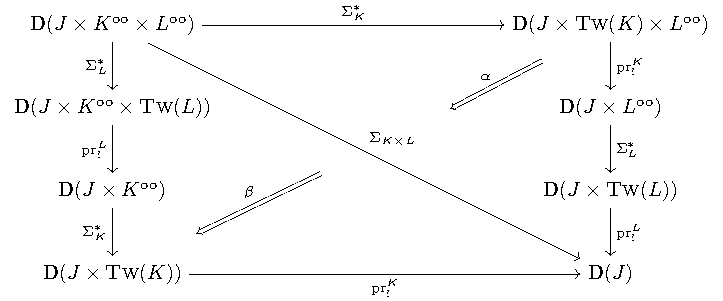
\includegraphics[scale=.75]{figures/fig11}
\end{center}
commutes for canonically determined 2-cells $\alpha$ and $\beta$.
\item \label{ex8:derivweighlim} State and prove an existence theorem for \emph{weighted colimits} in a derivator: given a bimorphism $\boxplus\colon (\D^{\Sets},\D)\to \D(I|-)$, we define the colimit of $X\in \D(J)$, weighted by $W\in \D^{\Sets}$ as the coend (in $\D$) $\int^J W\boxplus X$, \ie as the image of the pair $(W,X)$ under the composition
\[
\D^{\Sets}(J^\opp)\times \D(J) \xto{\cdot} \D(I|J^\opp\times J) \xto{\int^J}\D(I).
\]
\end{exercisepoints}
\end{exerciseset}